% !TEX TS-program = XeLaTeX
% !TEX encoding = UTF-8 Unicode

%%%%%%%%%%%%%%%%%%%%%%%%%%%%%%%%%%%%%%%%%%%%%%%%%%%%%%%%%%%%%%%%%%%%%% % 
% 
% 大连理工大学硕士论文 XeLaTeX 模版 —— 主文件 main.tex
% 版本:1.0
% 最后更新:2023.01.07
% 修改者:QuYue (E-mail: quyue1541@gmail.com)
% 编译环境:Overleaf + TeXLive 2022
% 原修改者:Yuri (E-mail: yuri_1985@163.com)
% 原修订者:whufanwei(E-mail: dutfanwei@qq.com)
% 
%%%%%%%%%%%%%%%%%%%%%%%%%%%%%%%%%%%%%%%%%%%%%%%%%%%%%%%%%%%%%%%%%%%%%% 
% \PassOptionsToPackage{quiet}{fontspec} % 让字体不再给出警告(解开注释的话可以达到零警告)
\documentclass[12pt, a4paper, openany, twoside]{book}

% 字体配置文件
% !TEX TS-program = XeLaTeX
% !TEX encoding = UTF-8 Unicode

%%%%%%%%%%%%%%%%%%%%%%%%%%%%%%%%%%%%%%%%%%%%%%%%%%%%%%%%%%%%%%%%%%%%%% 
% 
% 大连理工大学硕士论文 XeLaTeX 模版 —— 字体配置文件 fonts.tex
% 版本:1.0
% 最后更新:2023.01.07
% 修改者:QuYue (E-mail: quyue1541@gmail.com)
% 编译环境:Overleaf + TeXLive 2022
% 原修改者:Yuri (E-mail: yuri_1985@163.com)
% 原修订者:whufanwei(E-mail: dutfanwei@qq.com)
% 
%%%%%%%%%%%%%%%%%%%%%%%%%%%%%%%%%%%%%%%%%%%%%%%%%%%%%%%%%%%%%%%%%%%%%% 

% 英文字体设置特别推荐方案(Windows,需要安装 Adobe 字体),现代
\usepackage{fontspec}
\usepackage{xltxtra,xunicode}
\usepackage[CJKchecksingle,BoldFont]{xeCJK}

\usepackage{amsmath}
\usepackage{amssymb}
% \usepackage{mathspec}
\setmainfont[Mapping=tex-text]{Times New Roman}
\setsansfont[Mapping=tex-text]{Arial} 
\setmonofont[Path="fonts/consolas/", BoldFont={consolab.ttf},ItalicFont={consolai.ttf}, BoldItalicFont={consolaz.ttf}]{consola.ttf}
% \setmathfont{Times New Roman}


% 英文字体设置方案一(Windows,需要安装 LM10 字体),和 LaTeX 默认字体保持一致,经典
% \usepackage{amssymb}
% \usepackage{fontspec}
% \usepackage{amsmath}
% \usepackage[CJKnumber,CJKaddspaces,CJKchecksingle,BoldFont]{xeCJK}
% \usepackage{mathrsfs}   % 一种常用于定义泛函算子的花体字母,只有大写。
% \usepackage{bm}         % 处理数学公式中的黑斜体的宏包
% \setmainfont{LMRoman10-Regular}
% \setsansfont{LMSans10-Regular}
% \setmonofont{LMMono10-Regular}

% 英文字体设置方案二(Linux,使用自带 LM10 字体),和 LaTeX 默认字体保持一致,经典
% \usepackage{fontspec}
% \usepackage{amsmath,amssymb}
% \usepackage[CJKnumber,CJKaddspaces,CJKchecksingle,BoldFont]{xeCJK}
% \usepackage{mathrsfs}   % 一种常用于定义泛函算子的花体字母,只有大写。
% \usepackage{bm}         % 处理数学公式中的黑斜体的宏包
% \setmainfont{LMRoman10}
% \setsansfont{LMSans10}
% \setmonofont{LMMono10}

% 英文字体设置方案三(Linux,使用自带 Nimbus 字体),和 Word 模版字体保持一致,经典
% \usepackage{fontspec}
% \usepackage{mathptmx}
% \usepackage{amsmath,amssymb}
% \usepackage[CJKnumber,CJKaddspaces,CJKchecksingle,BoldFont]{xeCJK}
% \usepackage{mathrsfs}   % 一种常用于定义泛函算子的花体字母,只有大写。
% \usepackage{bm}         % 处理数学公式中的黑斜体的宏包
% \setmainfont{Nimbus Roman No9 L}
% \setsansfont{Nimbus Sans L}
% \setmonofont{Nimbus Mono L}

% 以下字体已被下载至fonts文件夹中
% 中文字体设置,使用的是 Adobe 字体,保证了在 Adobe Reader / Acrobat 下优秀的显示效果
\setCJKmainfont[Path="fonts/Adobe/", BoldFont={AdobeHeitiStd-Regular.otf}, ItalicFont={AdobeKaitiStd-Regular.otf}]{AdobeSongStd-Light.otf}
\setCJKsansfont[Path="fonts/Adobe/"]{AdobeHeitiStd-Regular.otf}
\setCJKmonofont[Path="fonts/Adobe/"]{AdobeFangsongStd-Regular}

% 定义字体名称,可在此添加自定义的字体
\setCJKfamilyfont{song}[Path="fonts/Adobe/"]{AdobeSongStd-Light.otf}
\setCJKfamilyfont{hei}[Path="fonts/Adobe/"]{AdobeHeitiStd-Regular.otf}
\setCJKfamilyfont{kai}[Path="fonts/Adobe/"]{AdobeKaitiStd-Regular.otf}
\setCJKfamilyfont{fs}[Path="fonts/Adobe/"]{AdobeFangsongStd-Regular}
\setCJKfamilyfont{xkai}[Path="fonts/"]{STXingKai.ttf}
\setCJKfamilyfont{hwxh}[Path="fonts/"]{STXiHei.ttf}
\setCJKfamilyfont{cambria}[Path="fonts/cambria/", BoldFont={cambriab.ttf},ItalicFont={cambriai.ttf}, BoldItalicFont={cambriaz.ttf}]{cambria.ttc}


% 自动调整中英文之间的空白
% \punctstyle{quanjiao}
\XeTeXlinebreaklocale "zh"      %中文断行
\XeTeXlinebreakskip = 0pt plus 1pt %1pt左右弹性间距
% 其他字体宏包


% 宏包配置文件
% !TEX TS-program = XeLaTeX
% !TEX encoding = UTF-8 Unicode

%%%%%%%%%%%%%%%%%%%%%%%%%%%%%%%%%%%%%%%%%%%%%%%%%%%%%%%%%%%%%%%%%%%% 
% 
% 大连理工大学硕士论文 XeLaTeX 模版 —— 宏包配置文件 packages.tex
% 版本:1.0
% 最后更新:2023.01.07
% 修改者:QuYue (E-mail: quyue1541@gmail.com)
% 编译环境:Overleaf + TeXLive 2022
% 原修改者:Yuri (E-mail: yuri_1985@163.com)
% 原修订者:whufanwei(E-mail: dutfanwei@qq.com)
%%%%%%%%%%%%%%%%%%%%%%%%%%%%%%%%%%%%%%%%%%%%%%%%%%%%%%%%%%%%%%%%%%%%% 

% 页面设置
\usepackage[body={16.1cm, 22.2cm}]{geometry}
\usepackage{indentfirst}                         % 首行缩进宏包
\usepackage[sf]{titlesec}                        % 控制标题的宏包
\usepackage{titletoc}                            % 控制目录的宏包
\usepackage{fancyhdr}                            % 自定义页眉页脚
\usepackage[perpage,symbol]{footmisc}            % 脚注控制
% \usepackage{layouts}                             % 打印当前页面格式的宏包
\usepackage{paralist}                            % 一种换行不缩进的列表格式,asparaenum,inparaenum 等
\usepackage[shortlabels]{enumitem}               % 列表格式
\usepackage{fancyvrb}                            % 原样输出
\usepackage[amsmath,thmmarks,hyperref]{ntheorem} % 定理类环境宏包
\usepackage{type1cm}                             % 控制字体的大小

% 表格处理
\usepackage{booktabs}   % 三线表
\usepackage{multirow}   % 表格多行处理
\usepackage{diagbox}    % 斜线表头
\usepackage{tabularx}   % 表格折行
\usepackage{siunitx}    % 国际单位,小数点对齐
% \sisetup{inter-unit-product = { }\cdot{ }} 

% 参考文献

% 图形相关
\usepackage{graphicx}            % 请在引用图片时务必给出后缀名
\usepackage[x11names]{xcolor}    % 支持彩色
\usepackage[below]{placeins}     % 浮动图形控制宏包
\usepackage{rotating}            % 图形和表格的控制
\usepackage{subfigure}           % 插入子图形
\usepackage[subfigure]{ccaption} % 插图表格的双语标题
\usepackage{setspace}            % 定制表格和图形的多行标题行距

% \usepackage[subfigure]{tocloft}


\usepackage{listings}         % 源代码展示
\lstset{%
  language=TeX,
  defaultdialect=empty,
  basicstyle=\ttfamily\small,
  backgroundcolor=\color{LightSteelBlue1},
  keywordstyle=\color{blue},
  showspaces=false,
  showstringspaces=false,
  showtabs=false,
  tabsize=2,breakatwhitespace=false,
  columns=flexible}

% 其他
\usepackage{calc}   % 在 tex 文件中具有一些计算功能,主要用在页面控制。
\usepackage[xetex,
bookmarksnumbered=true,
bookmarksopen=true,
colorlinks=true,
% pdfborder={0 0 1},
citecolor=blue,
linkcolor=blue,
anchorcolor=green,
urlcolor=magenta,
breaklinks=true,
CJKbookmarks=true,
]{hyperref}

% 参考文献
\usepackage[numbers,sort&compress,square,super]{natbib} %参考文献
\usepackage{hypernat}
\usepackage{bibentry}

% 算法流程图
\usepackage{algorithm}
\usepackage{algorithmicx}
\usepackage{algpseudocode}
\usepackage{amsmath}

\usepackage{colortbl} % table color












% 格式文件
% !TEX TS-program = XeLaTeX
% !TEX encoding = UTF-8 Unicode

%%%%%%%%%%%%%%%%%%%%%%%%%%%%%%%%%%%%%%%%%%%%%%%%%%%%%%%%%%%%%%%%%%%%%% 
% 
% 大连理工大学硕士论文 XeLaTeX 模版 —— 格式配置文件 format.tex
% 版本:1.0
% 最后更新:2023.01.07
% 修改者:QuYue (E-mail: quyue1541@gmail.com)
% 编译环境:Overleaf + TeXLive 2022
% 原修改者:Yuri (E-mail: yuri_1985@163.com)
% 原修订者:whufanwei(E-mail: dutfanwei@qq.com)
% 
%%%%%%%%%%%%%%%%%%%%%%%%%%%%%%%%%%%%%%%%%%%%%%%%%%%%%%%%%%%%%%%%%%%%%% 

%%%%%%%%%%%%%%%%%%%%%%%%%%%%%%%%%%%%%%%%%%%%%%%%%%%%%%%%%%%%%%%%%%%%%% 
% 页面设置
%%%%%%%%%%%%%%%%%%%%%%%%%%%%%%%%%%%%%%%%%%%%%%%%%%%%%%%%%%%%%%%%%%%%%% 
% A4 纸张
\setlength{\paperwidth}{21.0cm}
\setlength{\paperheight}{29.7cm}
% 设置正文尺寸大小
\setlength{\textwidth}{16.1cm}
\setlength{\textheight}{22.2cm}
% 设置正文区在正中间
\newlength \mymargin
\setlength{\mymargin}{(\paperwidth-\textwidth)/2}
\setlength{\oddsidemargin}{(\mymargin)-1in}
\setlength{\evensidemargin}{(\mymargin)-1in}
% 设置正文区偏移量,奇数页向右偏,偶数页向左偏
\newlength \myshift
\setlength{\myshift}{0.0cm}	% 双面打印的奇偶页偏移值,可根据需要修改,建议小于 0.5cm
\addtolength{\oddsidemargin}{\myshift}
\addtolength{\evensidemargin}{-\myshift}
% 页眉页脚相关距离设置
\setlength{\topmargin}{-0.05cm}
\setlength{\headheight}{0.50cm}
\setlength{\headsep}{0.90cm}
\setlength{\footskip}{1.47cm}
% 公式的精调
\allowdisplaybreaks[4]  % 可以让公式在排不下的时候分页排,这可避免页面有大段空白。

% 下面这组命令使浮动对象的缺省值稍微宽松一点,从而防止幅度
% 对象占据过多的文本页面,也可以防止在很大空白的浮动页上放置很小的图形。
\renewcommand{\topfraction}{0.9999999}
\renewcommand{\textfraction}{0.0000001}
\renewcommand{\floatpagefraction}{0.9999}

%%%%%%%%%%%%%%%%%%%%%%%%%%%%%%%%%%%%%%%%%%%%%%%%%%%%%%%%%%%%%%%%%%%%%% 
% 颜色
%%%%%%%%%%%%%%%%%%%%%%%%%%%%%%%%%%%%%%%%%%%%%%%%%%%%%%%%%%%%%%%%%%%%%% 
\newcommand{\zhangsan}[1]{{\color{red}#1}}
\newcommand{\wanglaowu}[1]{{\color{blue}#1}}

%%%%%%%%%%%%%%%%%%%%%%%%%%%%%%%%%%%%%%%%%%%%%%%%%%%%%%%%%%%%%%%%%%%%%% 
% 字体字号定义
%%%%%%%%%%%%%%%%%%%%%%%%%%%%%%%%%%%%%%%%%%%%%%%%%%%%%%%%%%%%%%%%%%%%%% 
% 字号
\newcommand{\yihao}{\fontsize{26pt}{39pt}\selectfont}	  % 一号,1.5  倍行距
\newcommand{\xiaoyi}{\fontsize{24pt}{30pt}\selectfont}  % 小一,1.25 倍行距
\newcommand{\erhao}{\fontsize{22pt}{27.5pt}\selectfont} % 二号,1.25 倍行距
\newcommand{\xiaoer}{\fontsize{18pt}{22.5pt}\selectfont}% 小二,1.25 倍行距
\newcommand{\sanhao}{\fontsize{16pt}{20pt}\selectfont}  % 三号,1.25 倍行距
\newcommand{\xiaosan}{\fontsize{15pt}{19pt}\selectfont} % 小三,1.25 倍行距
\newcommand{\sihao}{\fontsize{14pt}{17.5pt}\selectfont} % 四号,1.25倍行距
\newcommand{\xiaosi}{\fontsize{12pt}{15pt}\selectfont}  % 小四,1.25倍行距
\newcommand{\dawu}{\fontsize{10.5pt}{18pt}\selectfont}  % 五号,1.75倍行距
\newcommand{\zhongwu}{\fontsize{10.5pt}{16pt}\selectfont}% 五号,1.5 倍行距
\newcommand{\wuhao}{\fontsize{10.5pt}{10.5pt}\selectfont}% 五号,单倍行距
\newcommand{\xiaowu}{\fontsize{9pt}{9pt}\selectfont}	   % 小五,单倍行距

\newcommand{\song}{\CJKfamily{song}} % 宋体
\newcommand{\hei}{\CJKfamily{hei}}   % 黑体
\newcommand{\kai}{\CJKfamily{kai}}   % 楷体
\newcommand{\fs}{\CJKfamily{fs}}     % 仿宋
\newcommand{\xkai}{\CJKfamily{xkai}} % 华文行楷
\newcommand{\hwxh}{\CJKfamily{hwxh}} % 华文细黑


% defaultfont 默认字体命令
\def\defaultfont{\renewcommand{\baselinestretch}{1.27}
  \fontsize{12pt}{15pt}\selectfont}

% 设置目录字体和行间距
\def\defaultmenufont{\renewcommand{\baselinestretch}{1.22}
  \fontsize{12pt}{15pt}\selectfont}

% 链接没有颜色(即目录是黑色,参考文献也是黑色)
\hypersetup{colorlinks=true,linkcolor=black,citecolor=black}

% 固定距离内容填入及下划线
\makeatletter
\newcommand\fixeddistanceleft[2][1cm]{{\hb@xt@ #1{#2\hss}}}
\newcommand\fixeddistancecenter[2][1cm]{{\hb@xt@ #1{\hss#2\hss}}}
\newcommand\fixeddistanceright[2][1cm]{{\hb@xt@ #1{\hss#2}}}
\newcommand\fixedunderlineleft[2][1cm]{\underline{\hb@xt@ #1{#2\hss}}}
\newcommand\fixedunderlinecenter[2][1cm]{\underline{\hb@xt@ #1{\hss#2\hss}}}
\newcommand\fixedunderlineright[2][1cm]{\underline{\hb@xt@ #1{\hss#2}}}
\makeatother

%%%%%%%%%%%%%%%%%%%%%%%%%%%%%%%%%%%%%%%%%%%%%%%%%%%%%%%%%%%%%%%%%%%%%% 
% 标题环境相关
%%%%%%%%%%%%%%%%%%%%%%%%%%%%%%%%%%%%%%%%%%%%%%%%%%%%%%%%%%%%%%%%%%%%%% 
% 定义、定理等环境
\theoremstyle{plain}
\theoremheaderfont{\hei\bf}
\theorembodyfont{\song\rmfamily}
\newtheorem{definition}{\hei 定义}[chapter]
\newtheorem{example}{\hei 例}[chapter]
%\newtheorem{algorithm}{\hei 算法}[chapter]
\newtheorem{theorem}{\hei 定理}[chapter]
\newtheorem{axiom}{\hei 公理}[chapter]
\newtheorem{proposition}[theorem]{\hei 命题}
\newtheorem{property}{\hei 性质}
\newtheorem{lemma}[theorem]{\hei 引理}
\newtheorem{corollary}{\hei 推论}[chapter]
\newtheorem{remark}{\hei 注解}[chapter]
\newtheorem{proof}{\hei 证明}[chapter]
% \newenvironment{proof}{\hei{证明} }{\hfill $\square$ \vskip 4mm}
% \setlength{\cftbeforetoctitleskip}{-0.25em}
% \setlength{\cftaftertoctitleskip}{0.25em}




% 目录标题
\renewcommand\contentsname{\xiaosan{\hfill 目  录\hfill}\vspace*{-1.25em}}
\renewcommand\listfigurename{\hfill 插~图~目~录 \hfill}
\renewcommand\listtablename{\hfill 表~格~目~录 \hfill}
\renewcommand{\bibname}{\hfill 参~考~文~献 \hfill}

%%%%%%%%%%%%%%%%%%%%%%%%%%%%%%%%%%%%%%%%%%%%%%%%%%%%%%%%%%%%%%%%%%%%%% 
% 段落章节相关
%%%%%%%%%%%%%%%%%%%%%%%%%%%%%%%%%%%%%%%%%%%%%%%%%%%%%%%%%%%%%%%%%%%%%% 
\setcounter{secnumdepth}{4}
\setcounter{tocdepth}{4}

\newcommand{\Cambria}{\CJKfamily{cambria}}

% 设置章、节、小节、小小节的间距
\titleformat{\chapter}[hang]{\normalfont\xiaosan\hei\sf}{\xiaosan\Cambria\thechapter}{1em}{\xiaosan}
\titlespacing{\chapter}{0pt}{-3ex  plus .1ex minus .2ex}{3.3ex}
\titleformat{\section}[hang]{\sihao\hei\sf}{\sihao\thesection}{1em}{}{}
\titlespacing{\section}{0pt}{0.5em}{0.5em}
\titleformat{\subsection}[hang]{\xiaosi\hei\sf}{\xiaosi\thesubsection}{1em}{}{}
\titlespacing{\subsection}{0pt}{0.5em}{0.3em}
\titleformat{\subsubsection}[hang]{\hei\sf}{\thesubsubsection}{1em}{}{}
\titlespacing{\subsubsection}{0pt}{0.3em}{0pt}
% 缩小目录中各级标题之间的缩进
\dottedcontents{chapter}[0.86cm+1.8em]{\vspace{0.0em}}{1.8em}{3pt}
\dottedcontents{section}[0.86cm+2.3em+2em]{}{2.3em}{3pt}
\dottedcontents{subsection}[0.86cm+3.1em+4em]{}{3.1em}{3pt}
\dottedcontents{subsubsection}[0.86cm+4em+6em]{}{4em}{3pt}
% \dottedcontents{chapter}[0.32cm]{\vspace{0.2em}}{1.0em}{5pt}
% \dottedcontents{section}[1.32cm]{}{1.8em}{5pt}
% \dottedcontents{subsection}[2.32cm]{}{2.7em}{5pt}
% \dottedcontents{subsubsection}[3.32cm]{}{3.4em}{5pt}
% 段落之间的竖直距离
\setlength{\parskip}{1.2pt}
% 段落缩进
\setlength{\parindent}{24pt}
% 定义行距
\renewcommand{\baselinestretch}{1.27}
% 参考文献条目间行间距
\setlength{\bibsep}{2pt}

%%%%%%%%%%%%%%%%%%%%%%%%%%%%%%%%%%%%%%%%%%%%%%%%%%%%%%%%%%%%%%%%%%%%%% 
% 页眉页脚设置
%%%%%%%%%%%%%%%%%%%%%%%%%%%%%%%%%%%%%%%%%%%%%%%%%%%%%%%%%%%%%%%%%%%%%% 


\newcommand{\makeheadrule}{%
  \makebox[0pt][l]{\rule[.7\baselineskip]{\headwidth}{0.75pt}}%
  \vskip-.8\baselineskip}

\makeatletter
\renewcommand{\headrule}{%
  {\if@fancyplain\let\headrulewidth\plainheadrulewidth\fi
    \makeheadrule}}

\pagestyle{fancyplain}

\fancyhf{}
\fancyhead[CO]{\song\wuhao{大连理工大学硕士学位论文}}
\fancyhead[CE]{\song\wuhao\@ctitle}
\fancyfoot[C,C]{\xiaowu$-$~\thepage~$-$}

\fancypagestyle{preContent}{ % 独创性声明的页眉
    \fancyhead{}
    \renewcommand\headrulewidth{0.75pt}
}

% Clear Header Style on the Last Empty Odd pages
\makeatletter
\def\cleardoublepage{\clearpage\if@twoside \ifodd\c@page\else%
  \hbox{}%
  \thispagestyle{empty}%              % Empty header styles
  \newpage%
  \if@twocolumn\hbox{}\newpage\fi\fi\fi}



%%%%%%%%%%%%%%%%%%%%%%%%%%%%%%%%%%%%%%%%%%%%%%%%%%%%%%%%%%%%%%%%%%%%%% 
% 列表环境设置
%%%%%%%%%%%%%%%%%%%%%%%%%%%%%%%%%%%%%%%%%%%%%%%%%%%%%%%%%%%%%%%%%%%%%% 
\setlist[enumerate]{(1),itemsep=-5pt,topsep=0mm,labelindent=\parindent,leftmargin=*}

%%%%%%%%%%%%%%%%%%%%%%%%%%%%%%%%%%%%%%%%%%%%%%%%%%%%%%%%%%%%%%%%%%%%%% 
% 算法流程图设置
%%%%%%%%%%%%%%%%%%%%%%%%%%%%%%%%%%%%%%%%%%%%%%%%%%%%%%%%%%%%%%%%%%%%%% 
\floatname{algorithm}{算法}
\renewcommand{\algorithmicrequire}{\textbf{输入:}}
\renewcommand{\algorithmicensure}{\textbf{输出:}}


%%%%%%%%%%%%%%%%%%%%%%%%%%%%%%%%%%%%%%%%%%%%%%%%%%%%%%%%%%%%%%%%%%%%%% 
% 国际单位,以点连接。s
%%%%%%%%%%%%%%%%%%%%%%%%%%%%%%%%%%%%%%%%%%%%%%%%%%%%%%%%%%%%%%%%%%%%%% 
\sisetup{inter-unit-product = { }\cdot{ }} 

%%%%%%%%%%%%%%%%%%%%%%%%%%%%%%%%%%%%%%%%%%%%%%%%%%%%%%%%%%%%%%%%%%%%%% 
% 参考文献的处理
%%%%%%%%%%%%%%%%%%%%%%%%%%%%%%%%%%%%%%%%%%%%%%%%%%%%%%%%%%%%%%%%%%%%%% 

% \addtolength{\bibsep}{-0.5em}              % 缩小参考文献间的垂直间距
\setlength{\bibhang}{2em}

\bibpunct{[}{]}{,}{s}{}{}

% \let\orig@Itemize =\itemize     
% \let\orig@Enumerate =\enumerate
% \let\orig@Description =\description

% \def\Myspacing{\itemsep=1ex \topsep=-4ex \partopsep=-2ex \parskip=-1ex \parsep=2ex}
% \def\newitemsep{
% \renewenvironment{itemize}{\orig@Itemize\Myspacing}{\endlist}
% \renewenvironment{enumerate}{\orig@Enumerate\Myspacing}{\endlist}
% \renewenvironment{description}{\orig@Description\Myspacing}{\endlist}
% }
%   \def\olditemsep{
%   \renewenvironment{itemize}{\orig@Itemize}{\endlist}
%   \renewenvironment{enumerate}{\orig@Enumerate}{\endlist}
%   \renewenvironment{description}{\orig@Description}{\endlist}
% }
%   \renewcommand{\labelenumi}{(\arabic{enumi})}
%   \newitemsep

%%%%%%%%%%%%%%%%%%%%%%%%%%%%%%%%%%%%%%%%%%%%%%%%%%%%%%%%%%%%%%%%%%%%%%   
%   其他设置
%%%%%%%%%%%%%%%%%%%%%%%%%%%%%%%%%%%%%%%%%%%%%%%%%%%%%%%%%%%%%%%%%%%%%%   
%   增加 \ucite 命令使显示的引用为上标形式
%   \newcommand{\ucite}[1]{$^{\mbox{\scriptsize \cite{#1}}}$}

%%%%%%%%%%%%%%%%%%%%%%%%%%%%%%%%%%%%%%%%%%%%%%%%%%%%%%%%%%%%%%%%%%%%%%   
%   图形表格
%%%%%%%%%%%%%%%%%%%%%%%%%%%%%%%%%%%%%%%%%%%%%%%%%%%%%%%%%%%%%%%%%%%%%%   
\renewcommand{\figurename}{图}
\renewcommand{\tablename}{表}
% \captionstyle{\centering}
% \hangcaption
\captiondelim{\hspace{1em}}
\captionnamefont{\zhongwu}
\captiontitlefont{\zhongwu}
\setlength{\abovecaptionskip}{0pt}
\setlength{\belowcaptionskip}{0pt}


\newcommand{\tablepage}[2]{\begin{minipage}{#1}\vspace{0.5ex} #2 \vspace{0.5ex}\end{minipage}}
\newcommand{\returnpage}[2]{\begin{minipage}{#1}\vspace{0.5ex} #2 \vspace{-1.5ex}\end{minipage}}


%%%%%%%%%%%%%%%%%%%%%%%%%%%%%%%%%%%%%%%%%%%%%%%%%%%%%%%%%%%%%%%%%%%%%% 
% 定义题头格言的格式
%%%%%%%%%%%%%%%%%%%%%%%%%%%%%%%%%%%%%%%%%%%%%%%%%%%%%%%%%%%%%%%%%%%%%% 

\newsavebox{\AphorismAuthor}
\newenvironment{Aphorism}[1]
{\vspace{0.5cm}\begin{sloppypar} \slshape
    \sbox{\AphorismAuthor}{#1}
    \begin{quote}\small\itshape }
    {\\ \hspace*{\fill}------\hspace{0.2cm} \usebox{\AphorismAuthor}
    \end{quote}
  \end{sloppypar}\vspace{0.5cm}}

% 自定义一个空命令,用于注释掉文本中不需要的部分。
\newcommand{\comment}[1]{}

% This is the flag for longer version
\newcommand{\longer}[2]{#1}

\newcommand{\ds}{\displaystyle}

% define graph scale
\def\gs{1.0}

%%%%%%%%%%%%%%%%%%%%%%%%%%%%%%%%%%%%%%%%%%%%%%%%%%%%%%%%%%%%%%%%%%%%%%%%%%%%%%%% 
% 封面摘要
%%%%%%%%%%%%%%%%%%%%%%%%%%%%%%%%%%%%%%%%%%%%%%%%%%%%%%%%%%%%%%%%%%%%%%%%%%%%%%%% 
\def\cdegree#1{\def\@cdegree{#1}}\def\@cdegree{}
\def\ctitle#1{\def\@ctitle{#1}}\def\@ctitle{}
\def\caffil#1{\def\@caffil{#1}}\def\@caffil{}
\def\csubject#1{\def\@csubject{#1}}\def\@csubject{}
\def\cauthor#1{\def\@cauthor{#1}}\def\@cauthor{}
\def\cauthorno#1{\def\@cauthorno{#1}}\def\@cauthorno{}
\def\csupervisor#1{\def\@csupervisor{#1}}\def\@csupervisor{}
\def\cdate#1{\def\@cdate{#1}}\def\@cdate{}
\long\def\cabstract#1{\long\def\@cabstract{#1}}\long\def\@cabstract{}
\def\ckeywords#1{\def\@ckeywords{#1}}\def\@ckeywords{}
\def\etitle#1{\def\@etitle{#1}}\def\@etitle{}
\long\def\eabstract#1{\long\def\@eabstract{#1}}\long\def\@eabstract{}
\def\ekeywords#1{\def\@ekeywords{#1}}\def\@ekeywords{}

% 封面
\def\makecover{
  \begin{titlepage}
    \newpage
    \thispagestyle{empty}
    \begin{center}
      \parbox[t][4.40cm][c]{\textwidth}
      {
        \begin{center}
          {\xiaoyi\song\textbf{\@cdegree}\\}
          \vspace{1.34cm}
          {\erhao\hwxh\textbf{\@ctitle}\\}
          \vspace{0.13cm}
          {\sanhao\textbf{\@etitle}\\}
        \end{center}
      }
      \parbox[b][10.39cm][c]{\textwidth}
      {
        \vspace{8.05cm}
        \begin{center}
          {
            \xiaosan\song
            \begin{tabular}{p{0.6cm}p{6.4em}@{\extracolsep{0.5em}}lc}
              \vspace{-0.41cm}
              ~ & 作 \hfill 者 \hfill 姓 \hfill 名:& \fixedunderlineleft[6.08cm]{\@cauthor} & \\
              \vspace{-0.41cm}
              ~ & 学 \hfill 科 \hfill 、\hfill 专 \hfill 业:& \fixedunderlineleft[6.08cm]{\@csubject} & \\
              \vspace{-0.41cm}
              ~ & 学 \hfill 号:& \fixedunderlineleft[6.08cm]{\@cauthorno} & \\
              \vspace{-0.41cm}
              ~ & 指 \hfill 导 \hfill 教 \hfill 师:& \fixedunderlineleft[6.08cm]{\@csupervisor} & \\
              \vspace{-0.41cm}
              ~ & 完 \hfill 成 \hfill 日 \hfill 期:& \fixedunderlineleft[6.08cm]{\@cdate} & \\
              \vspace{-0.41cm}
            \end{tabular}
          }
        \end{center}
      }
      
      \vspace{2.34cm}
      
      {
     	\xiaoer\xkai
        大连理工大学\\
        \vspace{0.24cm}
        \xiaosi\song
        Dalian University of Technology
      }
    \end{center}
    %\cleardoublepage
  \end{titlepage}
}

% 独创性说明
\def\originality{
  \renewcommand{\baselinestretch}{1.61}
  \newpage
  \thispagestyle{preContent}
  \begin{center}
    \parbox[t][1.52cm][c]{\textwidth}
    {\xiaoer\song\centerline{大连理工大学学位论文独创性声明}}
    \parbox[t][7.68cm][c]{\textwidth}
    {
      \sihao\fs\noindent
        作者郑重声明:所呈交的学位论文,是本人在导师的指导下进行研究工作所取得的成果。%
      尽我所知,除文中已经注明引用内容和致谢的地方外,%
      本论文不包含其他个人或集体已经发表的研究成果,%
      也不包含其他已申请学位或其他用途使用过的成果。%
      与我一同工作的同志对本研究所做的贡献均已在论文中做了明确的说明并表示了谢意。%
      
      \vspace{0.47cm}\noindent
        若有不实之处,本人愿意承担相关法律责任。
    }
    \parbox[t][0.58cm][c]{\textwidth}
    {\sihao\fs 学{\hfill}位{\hfill}论{\hfill}文{\hfill}题{\hfill}目{\hfill}:\fixedunderlinecenter[12.6cm]{\@ctitle}}
    \parbox[t][1.22cm][c]{\textwidth}
    {\sihao\fs 作{\hfill}者{\hfill}签{\hfill}名{\hfill}:\fixeddistanceleft[12.6cm]{\underline{\hspace{5.8cm}}\hfill
	日期:\underline{\hspace{1.4cm}}~年~{\underline{\hspace{0.7cm}}~月~{\underline{\hspace{0.7cm}}~日~}}}}
  \end{center}
  \renewcommand{\baselinestretch}{1.27}

  %\cleardoublepage
}

\def\authorization
{
  \begin{center}
    \sanhao\hei~大连理工大学学位论文版权使用授权书~
  \end{center}
  
  \sihao\fs\noindent
    本人完全了解学校有关学位论文知识产权的规定,%
  在校攻读学位期间论文工作的知识产权属于大连理工大学,允许论文被查阅和借阅。%
  学校有\linebreak 权保留论文并向国家有关部门或机构送交论文的复印件和电子版,%
  可以将本学位论文的全部或部分内容编入有关数据库进行检索,%
  可以采用影印、\linebreak 缩印、或扫描等复制手段保存和汇编本学位论文。%
  \\
  
  \vspace{0.2cm}\noindent
  学{\hfill}位{\hfill}论{\hfill}文{\hfill}题{\hfill}目{\hfill}:\fixedunderlinecenter[12.6cm]{\@ctitle}\\
  作{\hfill}者{\hfill}签{\hfill}名{\hfill}:\fixeddistanceleft[12.6cm]{\underline{\hspace{5.8cm}}\hfill
    日期:\underline{\hspace{1.4cm}}~年~{\underline{\hspace{0.7cm}}~月~{\underline{\hspace{0.7cm}}~日~}}}\\
  导{\hfill}师{\hfill}签{\hfill}名{\hfill}:\fixeddistanceleft[12.6cm]{\underline{\hspace{5.8cm}}\hfill
    日期:\underline{\hspace{1.4cm}}~年~{\underline{\hspace{0.7cm}}~月~{\underline{\hspace{0.7cm}}~日~}}}\\
  \renewcommand{\baselinestretch}{1.27}
}

\def\makeabstract{
  \defaultfont
  \chapter*{\hfill 摘  要 \hfill}
  \addcontentsline{toc}{chapter}{摘  要}
  \setcounter{page}{1}
  \@cabstract
  \vspace{0.53cm}
  
  \noindent {~~~~~~~~\hei{关键词:{\fs\@ckeywords}}}
  
  \defaultfont
  % \cleardoublepage
  \chapter*{}
  \addcontentsline{toc}{chapter}{Abstract}
  \vspace{-1.40cm}
  \begin{center}
    {\xiaosan\textrm{\@etitle}}
  \end{center}
  \vspace{-0.35cm}
  \begin{center}
    {
      \xiaosan{Abstract}\\
    }
  \end{center}
  \vspace{0.12cm}
  
  \@eabstract
  
  \vspace{0.55cm}
  
  \noindent {~~~~~~~~\textbf{Key Words:}}~~{\textsf{\@ekeywords}}
  %\cleardoublepage
}

\makeatletter
\def\hlinewd#1{%
  \noalign{\ifnum0=`}\fi\hrule \@height #1 \futurelet
  \reserved@a\@xhline}
\makeatother

% 定义索引生成
\def\generateindex
{
  \addcontentsline{toc}{chapter}{\indexname}
  \printindex
  %\cleardoublepage
}

\raggedbottom 
\begin{document}

% 定义所有的图片文件在 figures 子目录下
\graphicspath{{figures/}}

% 前言
\frontmatter
\pagenumbering{Roman}
% !TEX TS-program = XeLaTeX
% !TEX encoding = UTF-8 Unicode

%%%%%%%%%%%%%%%%%%%%%%%%%%%%%%%%%%%%%%%%%%%%%%%%%%%%%%%%%%%%%%%%%%%%%% 
% 
%	大连理工大学硕士论文 XeLaTeX 模版 —— 封面文件 cover.tex
%	版本:1.0
%	最后更新:2023.01.07
%   修改者:QuYue (E-mail: quyue1541@gmail.com)
%   编译环境:Overleaf + TeXLive 2022
%	原修改者:Yuri (E-mail: yuri_1985@163.com)
% 
%%%%%%%%%%%%%%%%%%%%%%%%%%%%%%%%%%%%%%%%%%%%%%%%%%%%%%%%%%%%%%%%%%%%%% 
\cdegree{硕~~士~~学~~位~~论~~文}
\ctitle{大连理工大学硕士学位论文模版}
\etitle{The \XeLaTeX{} Template of Master Degree Thesis  of DUT}

% 根据需要添加字符间距
\csubject{{\quad\;}~计算机科学与技术}
\cauthor{{\quad\;}~~~~~~~~~~~~~张三}
\cauthorno{{\quad\;}~~~~~~~~   20000000}
\csupervisor{{\quad\;}~~~~~~王老五~~~~教授 }

% 这里默认使用最后编译的时间,也可自行给定日期,注意汉字和数字之间的空格。
\cdate{{\quad\;}~~~\the\year~年~\the\month~月~\the\day~日}

\cabstract{
  本模版是根据大连理工大学硕士学位论文格式规范制作的硕士学位论文模板。
  
  本模板是基于北京大学、清华大学、哈尔滨工业大学等高校的硕博士论文模板,
  并按照大连理工大学硕士学位论文格式规范开发的论文模板,
  经过多人完善和修改,目前已经基本满足了论文规范的要求,
  而且易用性良好,功能强大。不过,可能还存在着一些问题,
  欢迎大家积极使用本模版,反馈遇到的问题,以便不断对其进行改进。
  
  当然这个模板仅仅是一个开始,希望有更多的人能够参与进来,
  不断改进准确性、易用性和较好的可维护性,造福需要的兄弟姐妹们。
  总体上来说,当前这个模板还是很值得推荐使用的。
  
  本模板的目的旨在推广这一优秀的排版软件在大工的应用,
  为广大同学提供一个方便、美观的论文模板,减少论文撰写格式方面的麻烦。

  和过去的版本不同的是,本版本的模板基本解决了过去版本存在相关的问题,并可以直接在overleaf上进行编辑,
  更为方便。
  
  以下顺便补充一些研究生院所提供的~Word~模版中的注意事项
  (略去已经嵌入到此模版中的内容):
    \begin{asparaenum}
  \item 论文摘要是学位论文的缩影,文字要简练、明确。内容要包括目的、方法、结果和结论。
    单位制一律换算成国际标准计量单位制,除特别情况外,数字一律用阿拉伯数码。
    文中不允许出现插图。重要的表格可以写入;
  \item 篇幅以一页为限,字数为~600-800~字
    (工程硕士、MBA、EMBA、MPA~等专业学位论文字数为~400-500~字);
  \item 摘要正文后,列出~3-5~个关键词。
    关键词请尽量用《汉语主题词表》等词表提供的规范词。
    关键词词间用分号间隔,末尾不加标点,3-5~个。
  \end{asparaenum}
}


\ckeywords{写作规范;排版格式;硕士学位论文;模版}

\eabstract{
  This is a template of master degree thesis of Dalian University of Technology,
  which is built according to the required format.
  
  内容应与“中文摘要”对应。使用第三人称,最好采用现在时态编写。
}

\ekeywords{Write Criterion; Typeset Format; Master's Degree Paper; Template}

\makecover   % 封面
\originality           % 独创性
\makeabstract

% 设置目录字体和行间距
\defaultmenufont
% 目录
\tableofcontents
% \cleardoublepage
% 插图目录
% \listoffigures
% 表格目录
% \listoftables
%\cleardoublepage

\defaultfont
\mainmatter
% 正文章节
\defaultfont
\renewcommand{\thefootnote}{\arabic{footnote}}
%\include{body/chap00} 引言部分删除
% !TEX TS-program = XeLaTeX
% !TEX encoding = UTF-8 Unicode

\chapter{绪论}
\label{chap01}
\section{研究背景}
为了方便在overleaf上写毕业论文,于是我在之前的模板的基础上制作本模板

这里我就写一下需要的配置好了。
为了方便在overleaf以及任意环境下使用,
已经提前下载好了必要的字体于"fonts"文件夹中。

在Overleaf中,需要配置的环境如下(已经默认配置好了,大家不要必就行):
\begin{enumerate}
\item 编译器 Compiler:XeLaTex
\item TexLive版本 Tex Live Version: 2022
\item 主文件 Main document: main.tex
\end{enumerate}

当然也可以下载至本地的环境来编译。


\subsection{绪论(或引言)内容要求}
以下给出研究生院对引言内容的要求,格式的要求已经嵌入到本模版中:
\begin{enumerate}
\item 绪论(或引言)包含的内容有说明论文的主题和选题的范围、对本论文研究主要范围内已有文献的评述以及
  说明本论文所要解决的问题;
\item 注意不要与摘要内容雷同;
\item 建议与相关历史回顾、前人工作的文献评论、理论分析等相结合,如果引言部分省略,
  该部分内容在正文中单独成章,标题改为绪论,用足够的文字叙述。
\end{enumerate}

\zhangsan
{特别注意:是否如实引用前人结果反映的是学术道德问题,应明确写出同行相近的和已取得的成果,避免抄袭之嫌。} 

\section{国内外研究现状}
\textbf{xx的研究}

...

\textbf{xx的研究}

...




\section{研究创新}

本文对于xx的问题,提出了xx算法,xx。本文的贡献如下:
% 贡献
\begin{itemize}
    \item 贡献1。
    \item 贡献2。
    \item 贡献3。
\end{itemize}

\section{本文的组织结构}
本文主要围绕着xx开展,并辅以模拟数据和真实数据的实验,来验证提出算法的合理性和有效性。

第一章主要针对文章的背景进行介绍,并对国内外已有的研究进行了总结,接着提出本文的创新点,最后展示文章的整体结构。

第二章主要介绍了xx...。

第三章主要介绍了xxxx。

在最后,本文会对当前的研究加以总结,指出算法的局限性,并对其后续的研究及改进方向提出了个人的建议。

% !TEX TS-program = XeLaTeX
% !TEX encoding = UTF-8 Unicode

\chapter{常用的结构}
\label{chap02}
\section{字体}
\textbf{加粗}
\emph{斜体}

\section{列表}
介绍一些列表
\subsection{有序列表}
\begin{enumerate}
    \item xx。
    \item xx。
    \item xx。
\end{enumerate}
\subsection{无序列表}
\begin{itemize}
    \item xx。
    \item xx。
    \item xx。
\end{itemize}


\section{图片}
图片要放入到 “figures”文件中,图片生成最好是用pdf格式(这样出来的图片中,文字是可以被选中的)

\subsection{图片普通引用}

如图\ref{fig:image1}所示,

其中[htbp]是调图片出现的位置,感叹号可以强制固定位置,具体的细节可以上网查询;

$\backslash$centering 是调图片的位置(这里是居中); 

$\backslash$includegraphics[scale=0.15]\{a-realtemplate.pdf\}中,scale是调图片大小,后面的a-realtemplate.pdf则是图片所在文件的名字(在figures文件夹中);

$\backslash$bicaption[fig:image1]\{单张图片\}\{单张图片\}\{Fig.\}\{One Images\}中,fig:image1是用来引用本图片的标签,想要引用的时候,只需要$\backslash$ref\{fig:image1\}就可以了,后面的则是图片的图片介绍以及中文说明和英文说明。

\begin{figure}[htbp]
  \centering
  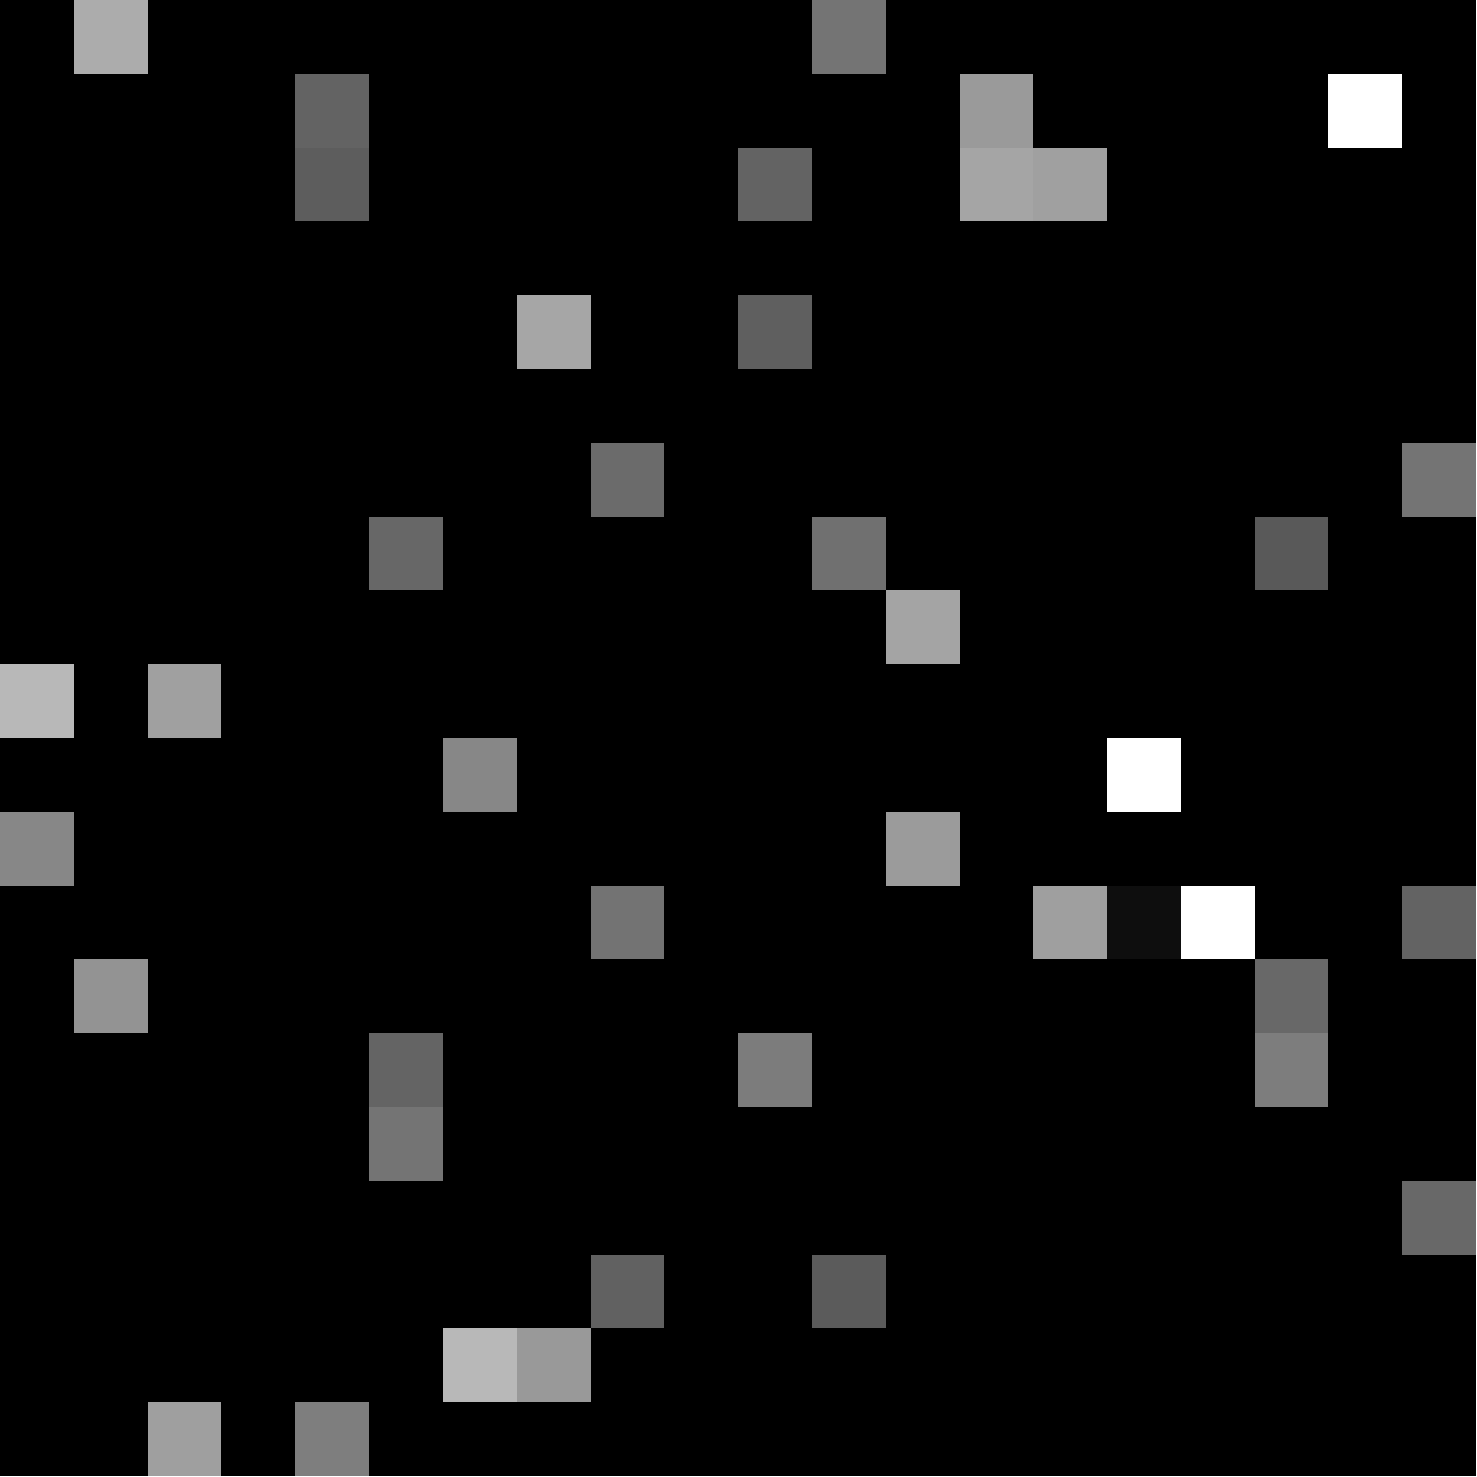
\includegraphics[scale=0.15]{a-realtemplate.pdf}
  \bicaption[fig:image1]{单张图片}{单张图片}{Fig.}{One Images}
\end{figure}

\subsection{多张图片引用}
如图\ref{fig:multi-images2}
\begin{figure}[t!]
  \centering
  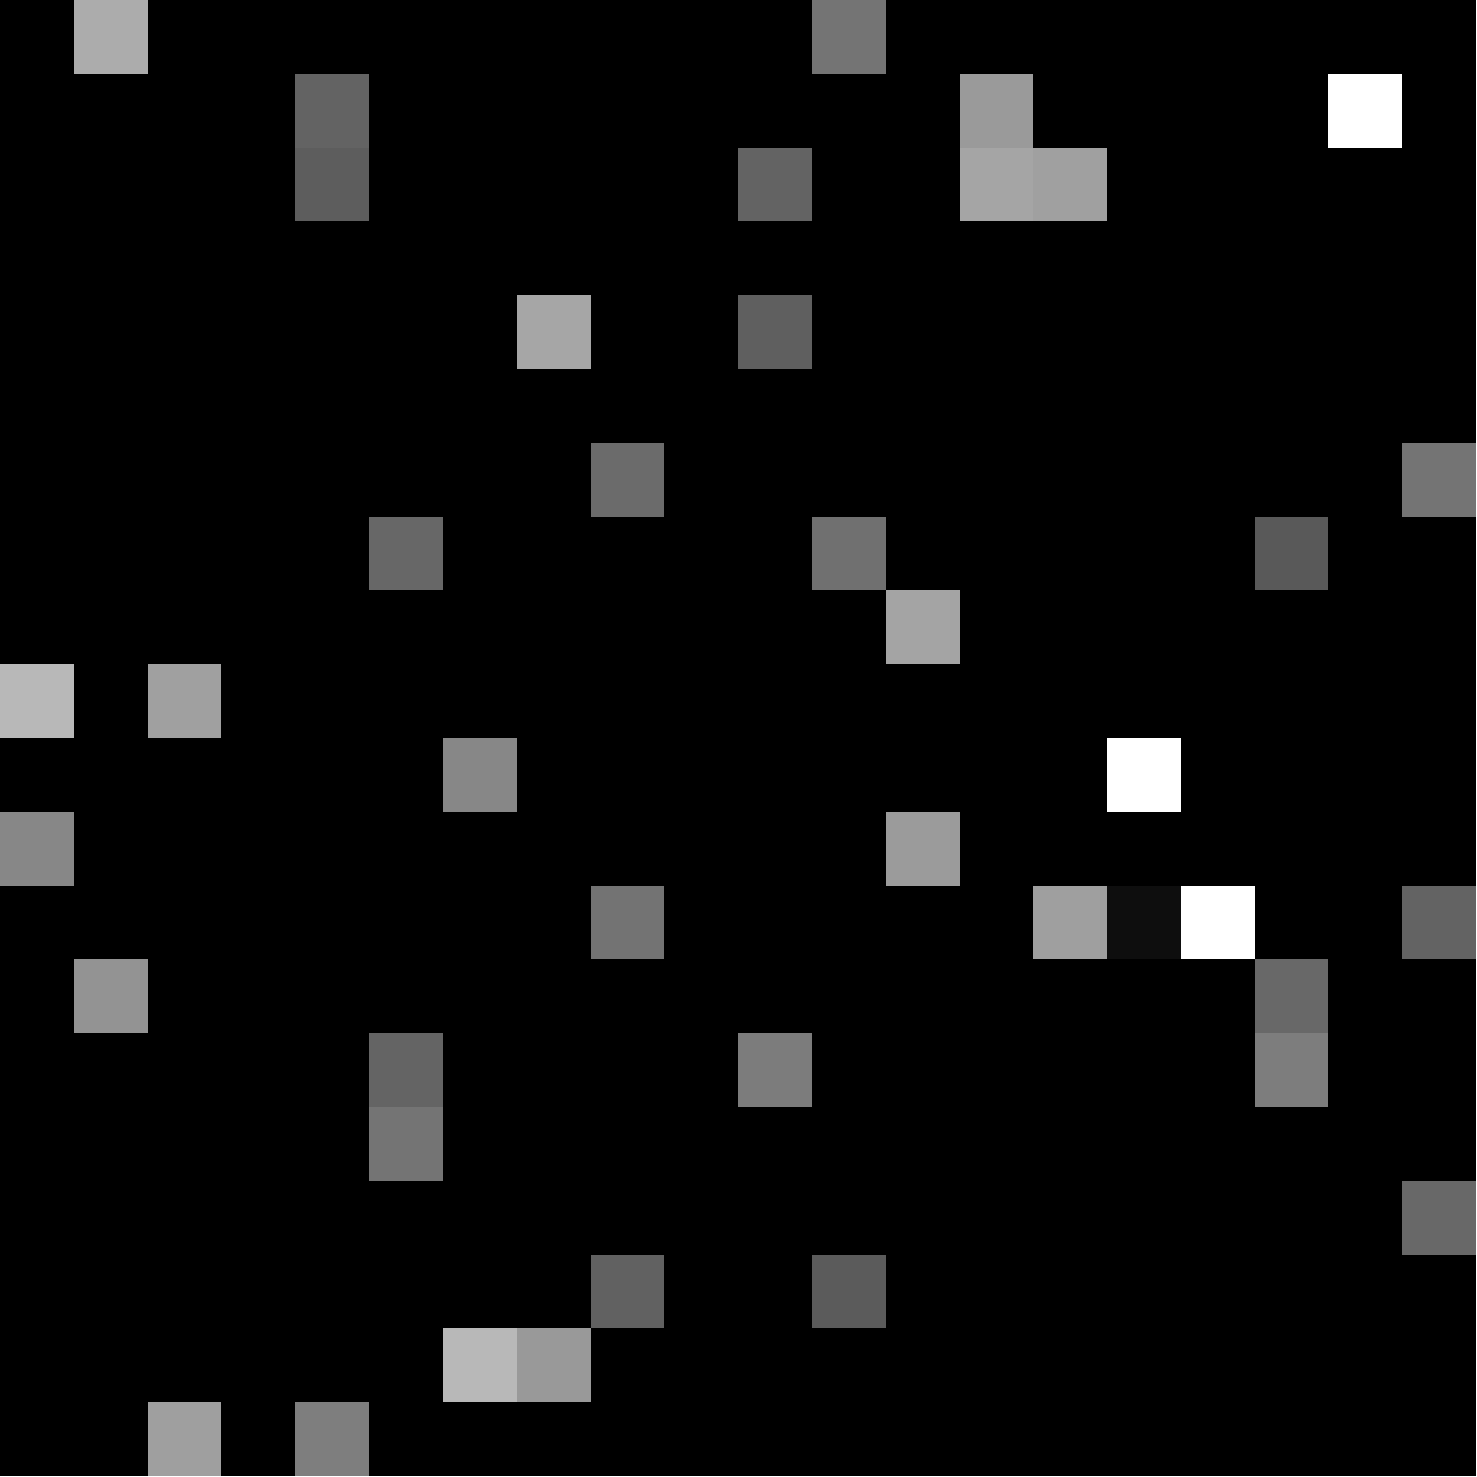
\includegraphics[width=0.2\linewidth]{a-realtemplate.pdf}
  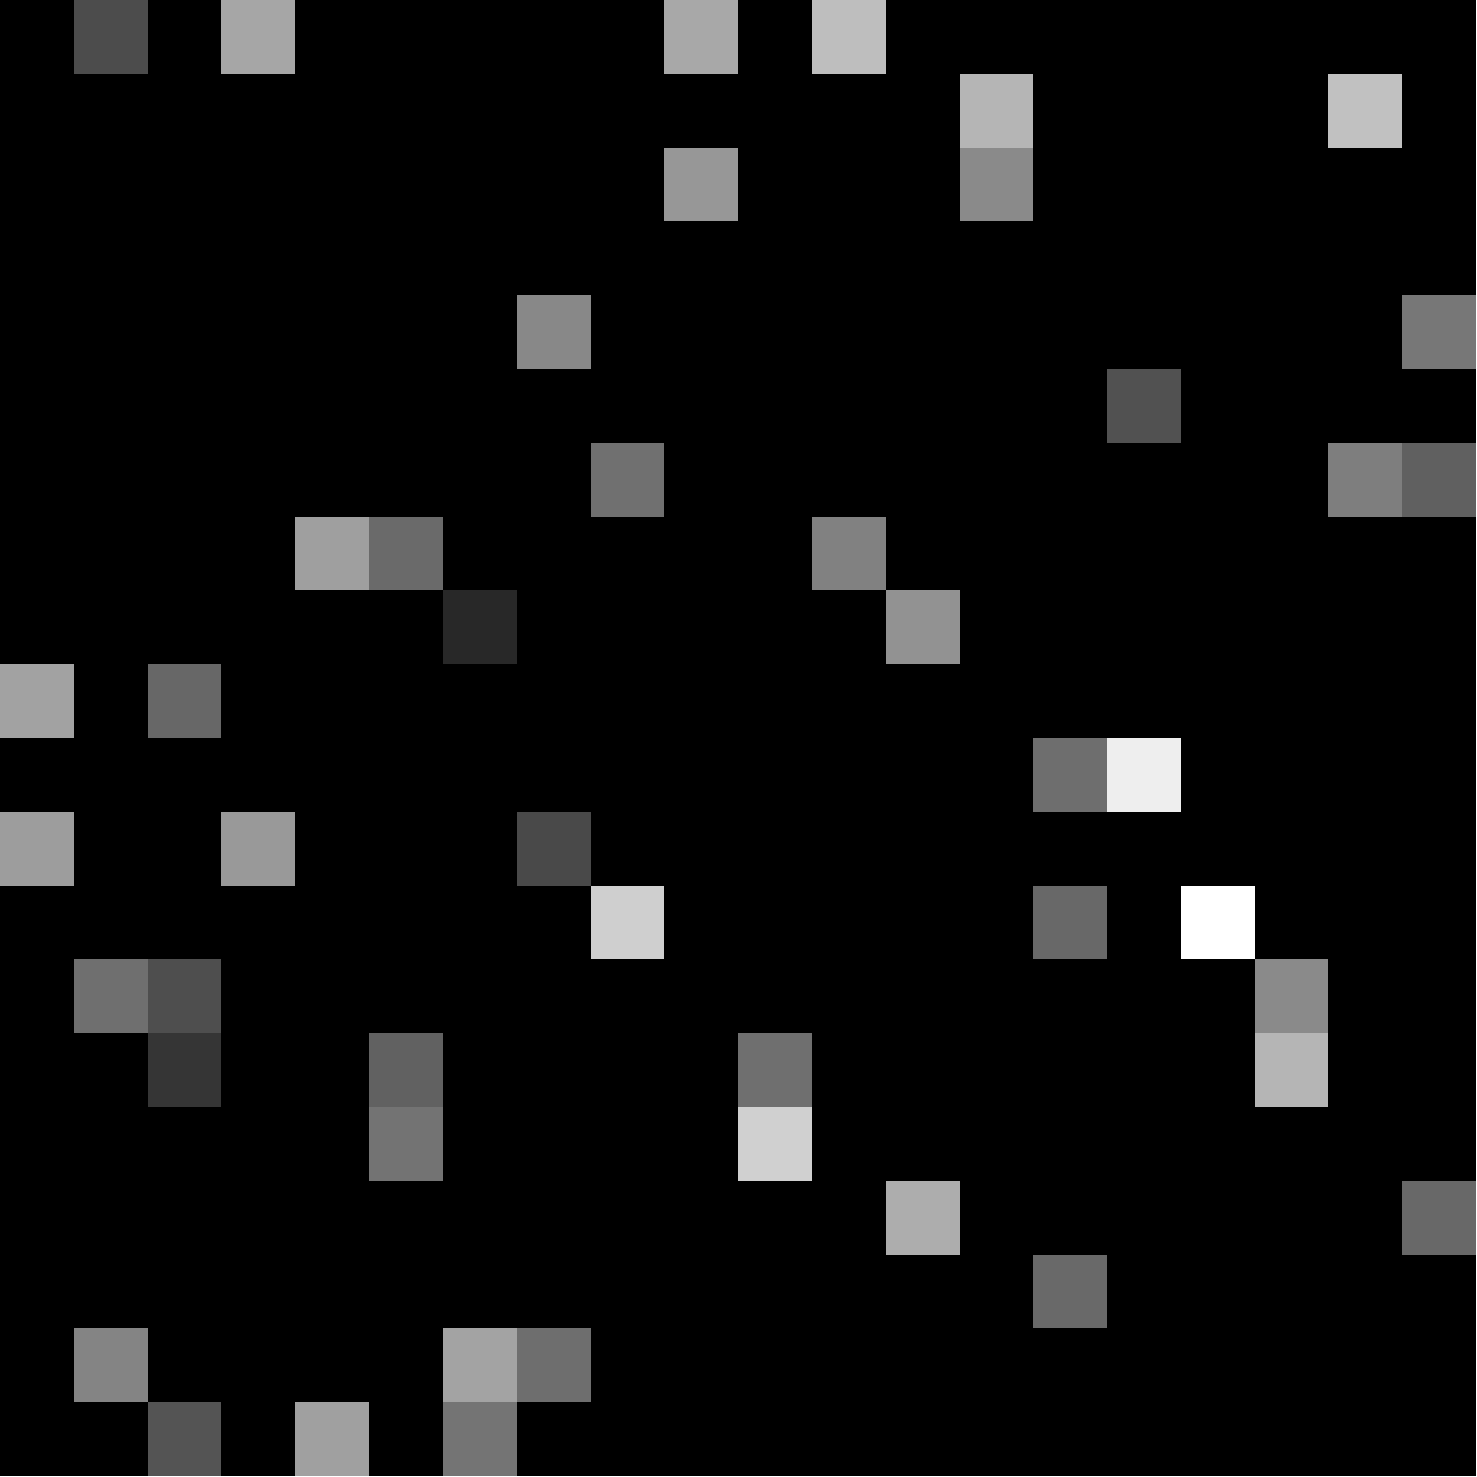
\includegraphics[width=0.2\linewidth]{b-computed-sparsity-template.pdf}
  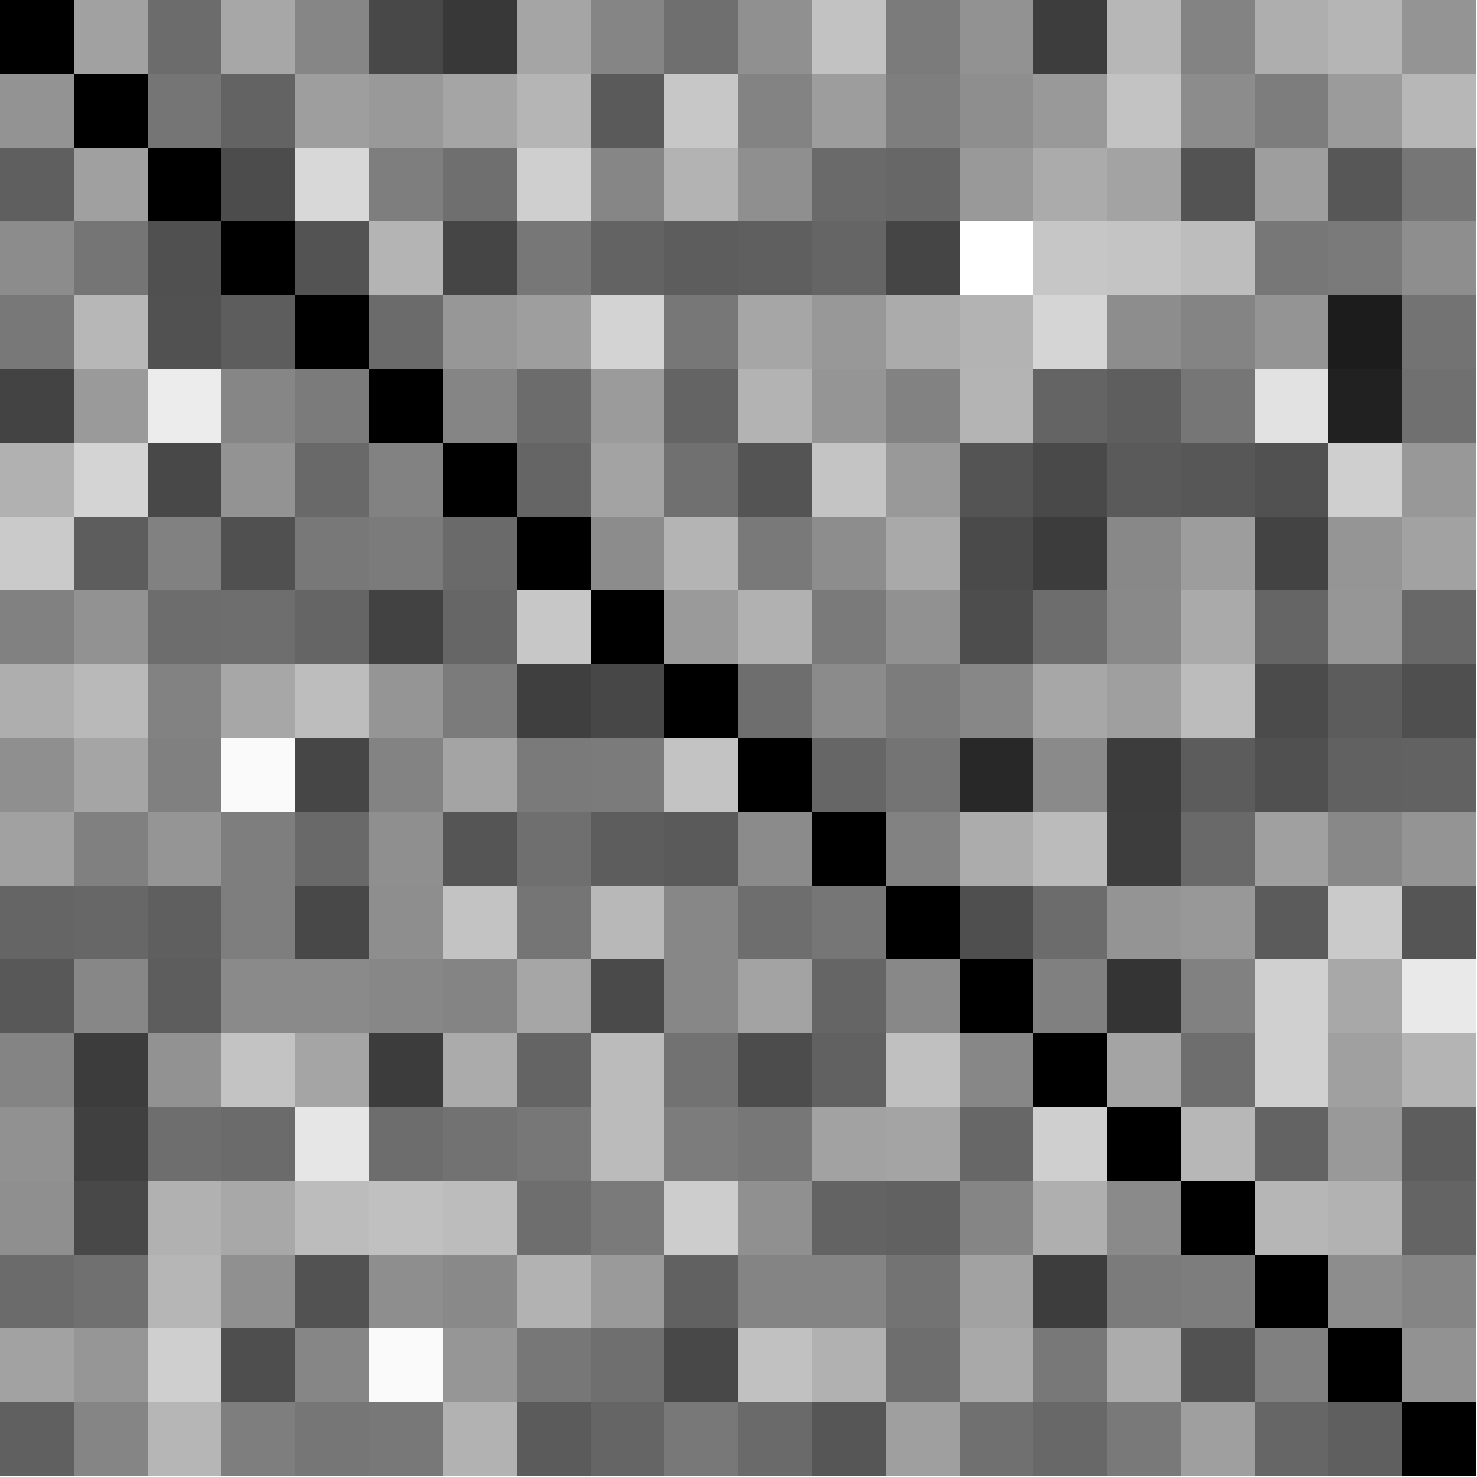
\includegraphics[width=0.2\linewidth]{c-real_template_without_template.pdf}
  \bicaption[fig:multi-images2]{RealTemplate}{多张图片}{Fig.}{Multiple Images}
\end{figure}


\section{表格}
\subsection{简单表格}
如表\ref{tab:datasets}所示。

\begin{table}[htbp]
  \bicaption[tab:datasets]{表}{数据集概览}{Tab.}{Summary of Datasets}
  \centering
  \vspace{0.2cm}
  \zhongwu
  \begin{tabular}{lcccccc}
  \toprule
  数据集 & 样本数量 & 记录数量 & 特征数量 & 平均记录数量 & 类别数 & $p/r$\\
  \midrule
  PPMI & 683 & 15798 & 212 & 23.1303 & 2 & 9/1 \\
  PS & 68 & 1208 & 26 & 17.7647 & 2 & 1.5/1 \\
  OD & 115 & 20560 & 5 & 178.7826 & 2 & 1/36 \\
  \bottomrule
  \end{tabular}
\end{table}

\subsection{复杂表格}
如表\ref{tab:Time}所示。

\begin{table*}[htbp]
  \bicaption[tab:Time]{表}{运行时间比较(秒)}{Tab.}{Comparisons of Running Time (in seconds)}
  \centering
  \vspace{0.2cm}
  \zhongwu
  \scalebox{0.85}[0.85]{
  \begin{tabular}{llcccccccccc}
  \toprule
  \multirow{2}{*}{Stage} & \multirow{2}{*}{Method} & \multicolumn{10}{c}{Number of Features} \\
  \cline{3-12}
   & & 20 & 40 & 60 & 80 & 100 & 120 & 140 & 160 & 180 & 200\\
  \midrule
  \multirow{7}{*}{Predicting} & PCC & 0.01 & 0.01 & 0.01 & 0.01 & 0.02 & 0.02 & 0.03 & 0.05 & 0.03 & 0.04 \\
  & PCC+Fisher & 0.02 & 0.01 & 0.02 & 0.01 & 0.03 & 0.04 & 0.02 & 0.04 & 0.05 & 0.06 \\
  & SR-C & 0.56 & 0.91 & 1.57 & 2.75 & 3.96 & 7.55 & 10.02 & 11.73 & 15.75 & 18.7\\
  & PINV & 0.03 & 0.02 & 0.02 & 0.06 & 0.05 & 0.07 & 0.08 & 0.09 & 0.08 & 0.10 \\
  & SR-PC & 1.51 & 1.52 & 1.54 & 1.56 & 1.64 & 1.64 & 1.77 & 1.77 & 2.01 & 1.83 \\
  & Reweight-L1 & 0.25 & 0.52 & 0.75 & 1.17 & 1.51 & 1.64 & 2.11 & 2.78 & 3.69 & 4.51 \\
  & SAR-noLC & 0.08 & 0.23 & 0.35 & 0.49 & 0.59 & 0.80 & 0.83 & 0.85 & 1.25 & 2.27 \\
  & \cellcolor[rgb]{.7,.8,.9}MNR & \cellcolor[rgb]{.7,.8,.9}34.96 & \cellcolor[rgb]{.7,.8,.9}110.05 & \cellcolor[rgb]{.7,.8,.9}208.64 & \cellcolor[rgb]{.7,.8,.9}331.16 & \cellcolor[rgb]{.7,.8,.9}541.52 & \cellcolor[rgb]{.7,.8,.9}762.71 & \cellcolor[rgb]{.7,.8,.9}1076.53 & \cellcolor[rgb]{.7,.8,.9}1373.08 & \cellcolor[rgb]{.7,.8,.9}1772.22 & \cellcolor[rgb]{.7,.8,.9}2078.27 \\
  & \cellcolor[rgb]{1,.9,.6}SAR & \cellcolor[rgb]{1,.9,.6}0.15 & \cellcolor[rgb]{1,.9,.6}0.25 & \cellcolor[rgb]{1,.9,.6}0.49 & \cellcolor[rgb]{1,.9,.6}0.36 & \cellcolor[rgb]{1,.9,.6}0.70 & \cellcolor[rgb]{1,.9,.6}0.94 & \cellcolor[rgb]{1,.9,.6}1.14 & \cellcolor[rgb]{1,.9,.6}1.12 & \cellcolor[rgb]{1,.9,.6}1.61 & \cellcolor[rgb]{1,.9,.6}2.48 \\
  \midrule
  \multirow{7}{*}{Training} & PCC & 0.35 & 0.55 & 1.28 & 1.80 & 3.58 & 6.31 & 8.90 & 13.16 & 17.17 & 18.45 \\
  & PCC+Fisher & 0.57 & 0.74 & 1.64 & 1.99 & 4.65 & 7.77 & 10.58 & 13.71 & 18.6 & 23.00 \\
  & SR-C & 3.07 & 11.33 & 19.57 & 33.7 & 50.29 & 109.33 & 146.78 & 215.24 & 222.99 & 248.01\\
  & PINV & 0.86 & 1.49 & 2.16 & 3.12 & 5.52 & 10.76 & 14.35 & 19.67 & 21.05 & 31.04\\
  & SR-PC & 14.77 & 10.72 & 13.27 & 16.47 & 21.64 & 27.51 & 33.53 & 38.52 & 47.09 & 51.69 \\
  & Reweight-L1 & 22.51 & 46.2 & 72.66 & 97.85 & 133.67 & 174.79 & 230.62 & 297.64 & 338.53 & 396.27 \\
  & SAR-noLC & 1.94 & 4.36 & 9.08 & 15.84 & 32.66 & 44.11 & 61.08 & 73.58 & 99.66 & 120.44 \\
  & \cellcolor[rgb]{.7,.8,.9}MNR & \cellcolor[rgb]{.7,.8,.9}7.80 & \cellcolor[rgb]{.7,.8,.9}22.06 & \cellcolor[rgb]{.7,.8,.9}43.65 & \cellcolor[rgb]{.7,.8,.9}68.19 & \cellcolor[rgb]{.7,.8,.9}109.42 & \cellcolor[rgb]{.7,.8,.9}159.80 & \cellcolor[rgb]{.7,.8,.9}220.61 & \cellcolor[rgb]{.7,.8,.9}285.08 & \cellcolor[rgb]{.7,.8,.9}369.83 & \cellcolor[rgb]{.7,.8,.9}426.79 \\
  & \cellcolor[rgb]{1,.9,.6}SAR & \cellcolor[rgb]{1,.9,.6}3.55 & \cellcolor[rgb]{1,.9,.6}6.95 & \cellcolor[rgb]{1,.9,.6}12.76 & \cellcolor[rgb]{1,.9,.6}21.33 & \cellcolor[rgb]{1,.9,.6}43.43 & \cellcolor[rgb]{1,.9,.6}56.08 & \cellcolor[rgb]{1,.9,.6}83.05 & \cellcolor[rgb]{1,.9,.6}100.66 & \cellcolor[rgb]{1,.9,.6}137.93 & \cellcolor[rgb]{1,.9,.6}162.27 \\
  \bottomrule
  \end{tabular}}
\end{table*}


\section{文献引用}
我们的文献需要以BibTeX的格式放入到”body“文件夹中的"reference.bib"文件中。具体大家可以去看一下这个文件就明白了。对应的BibTeX格式大多数的文献管理网站和系统都能获取。
例如:\\
@inproceedings\{vaswani2017attention,\\
  title=\{Attention is all you need\},\\
  author=\{Vaswani, Ashish and Shazeer, Noam and Parmar, Niki and Uszkoreit, Jakob and Jones, Llion and Gomez, Aidan N and Kaiser, \{\L\}ukasz and Polosukhin, Illia\},\\
  booktitle=\{Advances in neural information processing systems\},\\
  pages=\{5998--6008\},\\
  year=\{2017\}\\
\}

其中第一行的vaswani2017attention,就是该文献的引用标签,只需要使用$\backslash$cite\{vaswani2017attention\}就可以引用本文献,效果如下:
Transformer\cite{vaswani2017attention}。

当然也可以同时引用多篇文献,只需要$\backslash$cite\{label1, label2\},效果如下:自适应LASSO\cite{leng2006note,meinshausen2006high}。


\section{公式}
下面介绍公式:
\subsection{行内式}
行内式就是在段落中的公式,用\$y=f(x)\$即可,例如:

有样本$X\in \mathbb{R}^{T_n\times P}$的$P$个特征都满足中心性(centered)和标准化性(normalized),即$X^T_{*i}X_{*i}=1$,$i=1,2,\cdots,P$。

\subsection{行外式}
行内式就是单独在外的公式,例如:
\begin{equation}
  \centering
  \label{e:PCC}
  \beta^{(n)}_{ij}=PCC(X^{(n)}_{*i},X^{(n)}_{*j}) 
\end{equation}

其中“e:PCC”就是这个公式的标签,需要引用公式的时候,使用$\backslash$ref,例如:
$\beta$的计算方法如公式\ref{e:PCC}所示。


\subsection{多行行外式}
当然,可以行外式可以多行,用aligned来使用,用$\backslash\backslash$来分行,用\&来对齐,如公式\ref{e:PCC2}所示
\begin{equation}
  \centering
  \label{e:PCC2}
  \begin{aligned}
  \rho(x,y)&=PCC(x,y)\\
  &=\frac{n\sum{x_iy_i-\sum{x_i}\sum{y_i}}}{\sqrt{n\sum{x^2_i}-(\sum{x_i})^2}\sqrt{n\sum{y^2_i}-(\sum{y_i})^2}}
  \end{aligned}
\end{equation}

\subsection{多公式行外式}
同上
\begin{equation}
\label{e:mfunction}
\begin{aligned}
  Accuracy & = \frac{TP+TN}{P+N}
  \\
  Precision & = \frac{TP}{TP+FP}
  \\
  Recall &= \frac{TP}{TP+FN}
  \\
  F1 &= \frac{2\times TP}{2\times TP + FP + FN}
\end{aligned}
\end{equation}

更详细的可参考https://katex.org/docs/supported.html



\section{算法流程图}
对于算法,可以用algorithm来编写,例子如下:

SAR算法的详细过程可见算法\ref{a:SAR detail}。
\begin{algorithm}[htbp]
    \caption{Shared Adaptive Regularization(SAR)算法详细过程}
    \label{a:SAR detail}
    \begin{algorithmic}[1]
    \State 设置步长$0<\eta\leq 1$,以及步长的步长$0<d<1$。(实际我们使用的是$\eta=1$,$d=\frac{1}{2}$)
    \State 初始化连通网络$\beta^{(n)}(0)$,$\forall n$,让其值的分布为标准正态分布。
    \State 根据公式\ref{e:PCC}或公式xx,利用$\beta(0)$计算初始模板$w(0)$。
    \State 根据公式xx,通过数据集计算出$L$矩阵。
    \State 根据公式xx,通过数据以及$L$矩阵,计算出$Q^{(n)}$及$c^{(n)}$,$\forall n$
    \For{$t=1,2,\cdots,T$}
        \While{1} 

        \State 根据$\beta(t-1)$和$w(t-1)$得到$B(t-1)$,然后拉成向量$\vec{B}(t-1)$。
        \State $z=prox_{\eta,h}\left( \vec{B}(t-1)- \nabla J(\vec{B}(t-1))\right)$
        \State $\hat{J}=J\left(\vec{B}(t-1)\right)+\nabla J\left( \vec{B}(t-1)\right)^T\left(z-\vec{B}(t-1)\right)+\frac{1}{2\eta}\|z-\vec{B}(t-1)\|_2^2$
        \If{$J(z)\leq\hat{J}$}
        \State break
        \EndIf
        \State $\eta=d\times \eta$
        \EndWhile
    \State $\vec{B}(t)=z$
    \State 根据$\vec{B}(t)$得到$B(t)$
    \State 根据$B(t)$和$w(t-1)$计算出$\beta(t)$
    \State 根据公式xx,利用$\beta(t)$计算模板$w(t)$。
    \EndFor
    \State \Return{稀疏连通网络$\beta(T)$和共享正则模板$w(T)$。}
    \end{algorithmic}
  \end{algorithm}

另一种写法,可参照算法\ref{a:Re-weighted}。
\begin{algorithm}
  \caption{迭代求解Reweight-L1算法}
  \label{a:Re-weighted}
  \begin{algorithmic}[1] %每行显示行号
    \Require 初始权重值$\lambda_{ij}^{(n)}(0)=1$,$\forall i,j$,$n=1,2,\cdots,N$,其中$\lambda^{(n)}\in\mathbb{R}^{P \times P}$;数据集$\{X^{(n)}\} : n=1,\cdots,N\}$,其中$X^{(n)}\in\mathbb{R}^{T_n \times P}$;初始连通网络$\{\beta^{(n)}(0) : n=1,\cdots,N\}$,其中$\beta^{(n)}\in\mathbb{R}^{P \times P}$;
    \Ensure 最终权重值$\lambda^{(n)}(l_{max})$;最终连通网络$\beta^{(n)}(l_{max})$;
    \Function {$\rm Iterative~~Reweighting$}{$\lambda(0), X, \beta(0)$}
      \State 令$l$代表迭代次数,最大迭代次数设置为$l_{max}$,
      \While{迭代次数$l<l_{max}$}
        \State 先求解公式\ref{e:reweighted_L1_1},得到第$l$代$\beta^{(n)}$,$n=1,2,\cdots,N$:
        \begin{equation}
          \label{e:reweighted_L1_1}
        \beta^{(n)}(l)=\underset{\beta^{(n)}}{\operatorname{argmin}}\frac{1}{2}\left\|X^{(n)}\beta^{(n)}(l-1)-X^{(n)}\right\|_F^2+\sum_{ij}\left|\lambda^{(n)}_{ij}(l-1)\beta^{(n)}_{ij}(l-1)\right|
        \end{equation}
        \State 接着用公式xx更新权重,得到第$l$代$\lambda^{(n)}$,$n=1,2,\cdots,N$:
        \begin{equation}
          \label{e:reweighted_L1_2}
        \lambda^{(n)}_{ij}(l)=\frac{1}{|\beta_{ij}^{(n)}(l)|+\epsilon}
        \end{equation}
      \EndWhile
      \State \Return $\lambda^{(n)}(l_{max}),\beta^{(n)}(l_{max})$,$n=1,2,\cdots,N$
    \EndFunction
  \end{algorithmic}
\end{algorithm}

\section{定理证明等自制结构}

有的时候我们需要自制的结构,例如 \textbf{定理},\textbf{证明}等

可以去"setup"文件夹中,找到"format.tex"文件,在该文件中有”标题环境相关“这一段落,就可以改了,例如$\backslash$newtheorem\{proof\}\{$\backslash$hei 证明\}[chapter],就添加了”证明“这一种结构($\backslash$hei是指使用黑体),使用方法如下:

对于定理1的证明,可见证明\ref{pr:1}:
\begin{proof}
  \label{pr:1}
你的证明。
\end{proof}

\section{章节}
\begin{itemize}
    \item 对于章节,每个章节的内容放在了"body"文件夹中的对应文件。
    \item 每一章,用$\backslash$chapter\{章的名字\}。
    \item 每一节,用$\backslash$section\{节的名字\}。
    \item 每一小节,用$\backslash$subsection\{小节的名字\}。
    \item 每一小小节,用$\backslash$subsubsection\{小小节的名字\},依次类推。
    \item 如何想要引用某一章节,可以在对应章节的下面,加上$\backslash$label\{你定义的label\},如:在第\ref{chap03}章中,第\ref{section03-01}节说到xxx。
\end{itemize}

\section{其它颜色字体}
如果有人想要对论文进行修改和评论的时候,可以使用其它的颜色的字体,可以在”setup“文件夹中的”颜色"部分,新增一下命令:

例如:

张三:

$\backslash$newcommand\{$\backslash$zhangsan\}[1]\{\{$\backslash$color\{red\}\#1\}\}

王老五:

$\backslash$newcommand\{$\backslash$wanglaowu\}[1]\{\{$\backslash$color\{blue\}\#1\}\}

效果如下:

\zhangsan{这一段我觉得写的不好,找个时间和老师商量一下}

\wanglaowu{可以看一下这个资料}




% !TEX TS-program = XeLaTeX
% !TEX encoding = UTF-8 Unicode

\chapter{第三章}
\label{chap03}


\section{第三章的第一节}
\label{section03-01}





%\include{body/chap04}
% 结论
% !TEX TS-program = XeLaTeX
% !TEX encoding = UTF-8 Unicode

\chapter*{\hfill 结  论 \hfill}
\addcontentsline{toc}{chapter}{结  论}

结论是理论分析和实验结果的逻辑发展,是整篇论文的归宿。
结论是在理论分析、试验结果的基础上,经过分析、推理、判断、归纳的过程而形成的总观点。
结论必须完整、准确、鲜明、并突出与前人不同的新见解。
% \cleardoublepage
% \backmatter


% 参考文献
\defaultfont
\wuhao
\bibliographystyle{zjugbno}
\bibliography{body/reference}
\addcontentsline{toc}{chapter}{参考文献}
% \cleardoublepage
% 附录
\defaultfont
\begin{appendix}
  % !TEX TS-program = XeLaTeX
% !TEX encoding = UTF-8 Unicode
%%%%%%%%%%%%%%%%%%%%%%%%%%%%%%%%%%%%%%%%%%%%%%%%%%%%%%%%%%%%%%%%%%%%% 
% 
%	大连理工大学硕士论文 XeLaTeX 模版 —— 附录A chapA.tex
%	版本:1.0
%	最后更新:2023.01.07
%   修改者:QuYue (E-mail: quyue1541@gmail.com)
%   编译环境:Overleaf + TeXLive 2022
%	原修改者:Yuri (E-mail: yuri_1985@163.com)
% 
%%%%%%%%%%%%%%%%%%%%%%%%%%%%%%%%%%%%%%%%%%%%%%%%%%%%%%%%%%%%%%%%%%%%% 
\chapter*{\hfill 附录~A 附录内容名称 \hfill}
\addcontentsline{toc}{chapter}{附录~A 附录内容名称}

以下内容可放在附录之内:

\begin{enumerate}[1.]
\item 正文内过于冗长的公式推导;
\item 方便他人阅读所需的辅助性数学工具或表格;
\item 重复性数据和图表;
\item 论文使用的主要符号的意义和单位;
\item 程序说明和程序全文。
\end{enumerate}

这部分内容可省略。






\end{appendix}
% \cleardoublepage

\defaultfont
% 发表的文章列表
% !TEX TS-program = XeLaTeX
% !TEX encoding = UTF-8 Unicode

%%%%%%%%%%%%%%%%%%%%%%%%%%%%%%%%%%%%%%%%%%%%%%%%%%%%%%%%%%%%%%%%%%%%% 
% 
% 大连理工大学硕士论文 XeLaTeX 模版 —— 发表论文文件 publications.tex
%	版本:1.0
%	最后更新:2023.01.07
%   修改者:QuYue (E-mail: quyue1541@gmail.com)
%   编译环境:Overleaf + TeXLive 2022
%	原修改者:Yuri (E-mail: yuri_1985@163.com)
% 
%%%%%%%%%%%%%%%%%%%%%%%%%%%%%%%%%%%%%%%%%%%%%%%%%%%%%%%%%%%%%%%%%%%%% 

\chapter*{\hfill 攻读硕士学位期间发表学术论文情况 \hfill}
\addcontentsline{toc}{chapter}{攻读硕士学位期间发表学术论文情况}
\begin{enumerate}[label={[\arabic*]}]
\item {\song\bf 作者1}, 作者2. 论文题目. 大连理工大学网络学刊,~2010年. 主
  办单位:~大连理工大学研究生院.~(本硕士学位论文第X章)
\end{enumerate}
% \cleardoublepage
% 致谢
% !TEX TS-program = XeLaTeX
% !TEX encoding = UTF-8 Unicode

%%%%%%%%%%%%%%%%%%%%%%%%%%%%%%%%%%%%%%%%%%%%%%%%%%%%%%%%%%%%%%%%%%%%% 
% 
%	大连理工大学硕士论文 XeLaTeX 模版 —— 致谢文件 acknowledgements.tex
%	版本:1.0
%	最后更新:2023.01.07
%   修改者:QuYue (E-mail: quyue1541@gmail.com)
%   编译环境:Overleaf + TeXLive 2022
%	原修改者:Yuri (E-mail: yuri_1985@163.com)
% 
%%%%%%%%%%%%%%%%%%%%%%%%%%%%%%%%%%%%%%%%%%%%%%%%%%%%%%%%%%%%%%%%%%%%% 

\chapter*{\hfill 致  谢 \hfill}
\addcontentsline{toc}{chapter}{致  谢}

学位论文中不得书写与论文工作无关的人和事,对导师的致谢要实事求是。

一同工作的同志对本研究所做的贡献应在论文中做明确的说明并表示谢意。

这部分内容不可省略。

在这里,向原作者和修改测试的同学、朋友表示感谢。





% \cleardoublepage
% 授权书
\chapter*{}
\addcontentsline{toc}{chapter}{大连理工大学学位论文版权使用授权书}
\renewcommand{\baselinestretch}{1.61}
\vspace{-0.48cm}
\authorization
% \cleardoublepage


\end{document}
